\section{ Принципы работы телескопов в разных диапазонах спектра. Наблюдения с поверхности Земли.}

Будем рассматривать только наблюдения с Земли, потому что про наблюдения из космоса весь второй билет.

\subsection{Оптический диапазон}

Телескоп представляет собой трубу (сплошную или каркасную), которая установлена на монтировке (бывает экваториальная и азимутальная, в зависимости от того, по каким осям двигается). Визуально имеет объектив (в который свет падает) и окуляр (в который смотрят глазом).

\subsubsection{Телескоп-рефрактор}

У рефракторов объективом является система линз.

Рефрактор исторически был создан раньше всех. Состоит из двух линз (объектив и окуляр), фокусы которых совмещены. Типичная схема приведена на рисунке \ref{fig:1_refractor}. Требует большой длины трубы, из-за чего неудобный.

\begin{figure}[H]
	\centering
	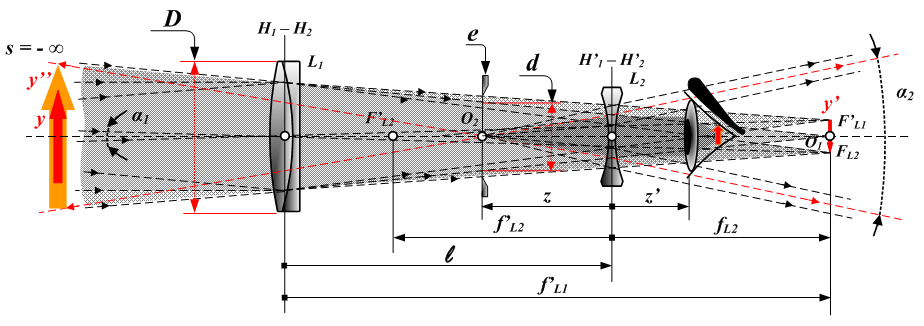
\includegraphics[width=0.7\linewidth]{1_refractor}
	\caption{Схема хода лучей в рефракторе Галилея}
	\label{fig:1_refractor}
\end{figure}

\subsubsection{Телескоп-рефлектор}

У рефлекторов объективом является вогнутое зеркало.

Появился несколько позже чем рефрактор, когда мы научились делать хорошие зеркала (не-металлические, поскольку металлические необходимо было часто шлифовать, поскольку они тускнели). Удобнее рефрактора тем, что большая часть массы сосредоточена ''внизу'' телескопа, что делает его удобнее в использовании. Типичная схема приведена на рисунке \ref{fig:1_reflector}.

\begin{figure}[H]
	\centering
	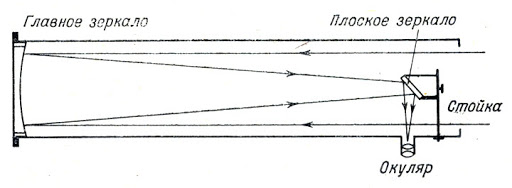
\includegraphics[width=0.7\linewidth]{1_reflector}
	\caption{Схема хода лучей в рефлекторе}
	\label{fig:1_reflector}
\end{figure}

Линза массивный объект, поскольку она сплошная, зеркало же работает поверхностью, поэтому оно менее массивное и удобнее. Кроме того, свет ходит туда-сюда, поэтому трубу можно делать короче. Короче сплошные плюсы.

\subsection{Радио-диапазон}

Радиотелескопы работают антенной, который бывают тарелками (как рефлекторы, т.е. огромная антенна фокусирует излучение на чувствительном приемнике, который далее преобразует его в удобную форму), и рогульками (такие например в Пущино стоят).

Для телескопов нам важны две характеристики: разрешающая способность и чувствительность. Для чувствительности нам нужна площадь антенны (есть прямая пропорциональность), а для разрешения --- максимальный размер антенны. Отсюда сразу понятно, что обычные параболические антенны дадут при фиксированной площади худшее разрешение. Поэтому мы можем сделать дырку в апертуре (но чтобы дырка была больше длины волны), при этом не потеряв в разрешении (а мы часто за ним и гоняемся).

По такому принципу, например, существует телескоп РАТАН-600 (см. рисунок \ref{fig:1_ratan}).

\begin{figure}[H]
	\centering
	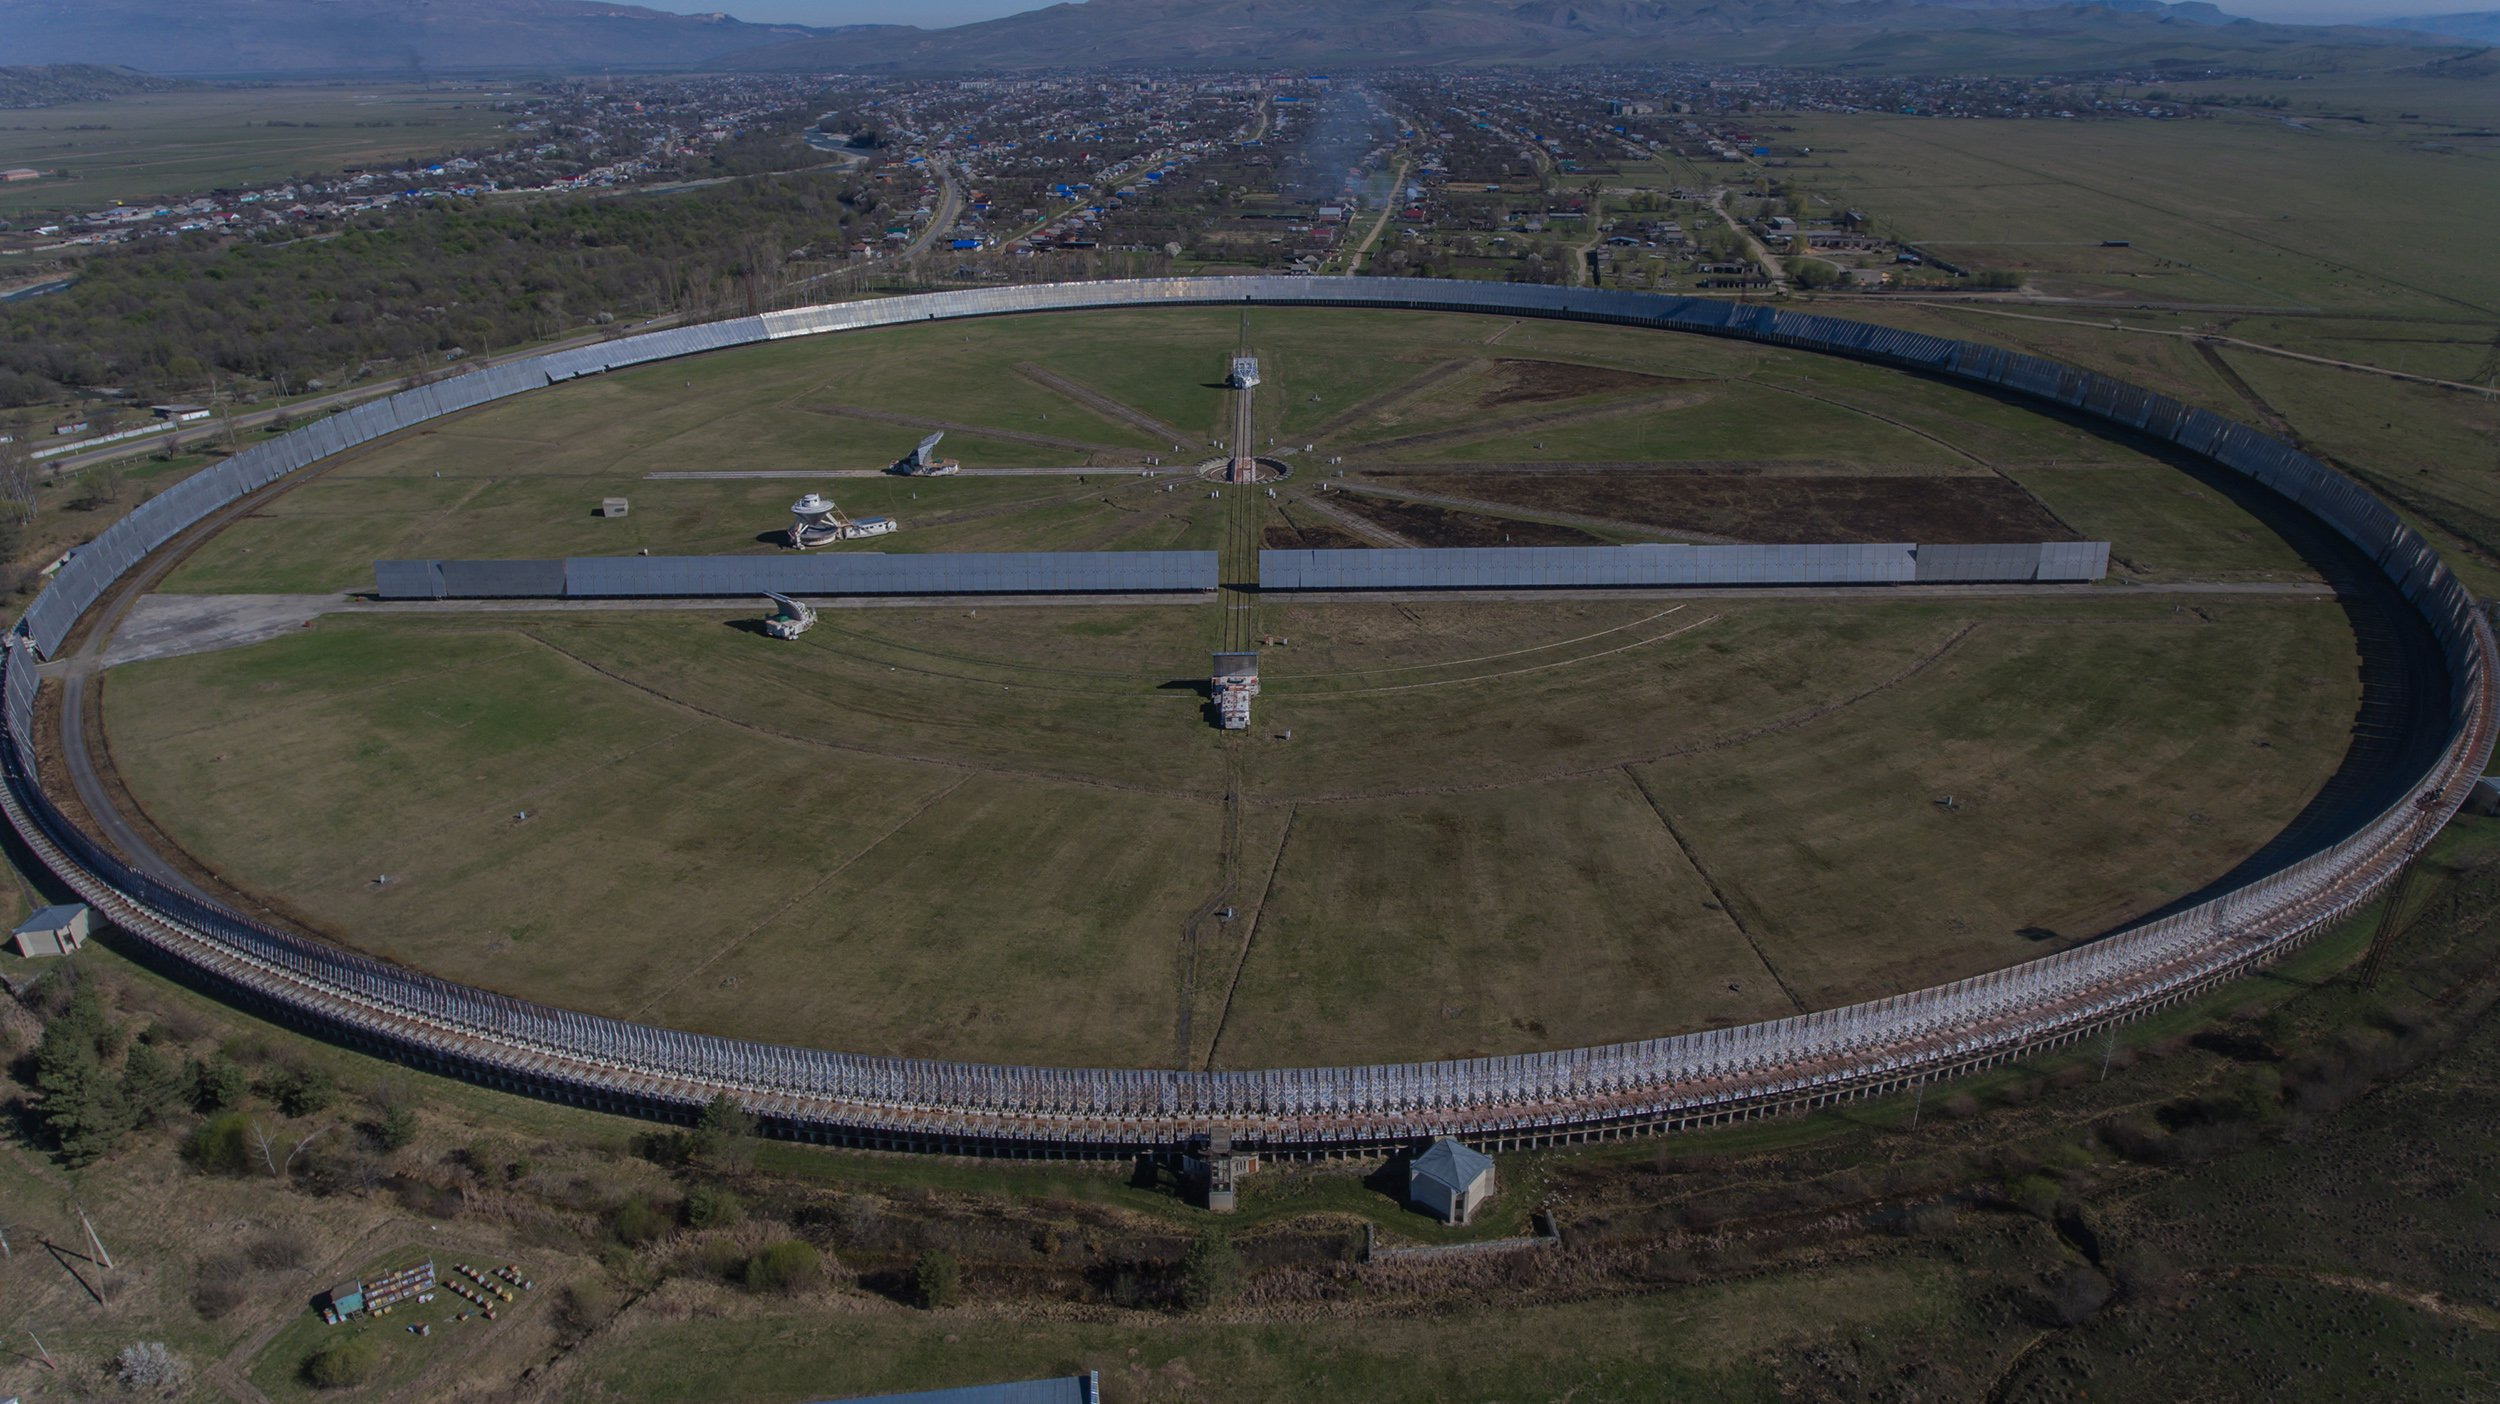
\includegraphics[width=0.7\linewidth]{1_ratan}
	\caption{РАТАН-600}
	\label{fig:1_ratan}
\end{figure}

Кроме того, мы можем взять не один огромный телескоп, а два (или больше) маленьких (это будет называться интерферометрами), но разнести их на большое расстояние друг от друга (например, так работал телескоп горизонта событий, на который получили недавние данные о черной дыре в M87). Работает из-за того что радиотелескопы работают на большой длине волны (низкой частоте). Мы обрабатываем данные вместе, и получается что у нас огромная база, дающая большое угловое разрешение (но на собирающей способности это выигрыша конечно не дает).

\subsection{Гамма-диапазон}

Проблема тут в том, что на Земле гамму не померить (не пропускает атмосфера). Но выход есть, можно регистрировать эффект, называемый \textbf{излучением Черенкова}, когда влетая в атмосферу Земли, гамма квант очень высокой энергии приводит к появлению вспышки в оптическом диапазоне. Нам нужны большие оптические телескопы для этого. Собрав фотоны мы получаем энергию кванта и направление, откуда он прилетел (с так себе точностью на самом деле).

\subsection{Космические лучи}

Космические лучи есть потоки частиц (электронов, протонов и более тяжелых ядер, а также их античастиц), распространяющихся в космическом пространстве.

Первичные (космические) заряженные частицы практически не достигают поверхности Земли, поэтому работают лишь косвенные методы наземной регистрации вторичных частиц и излучения. Методы регистрации космических лучей во многом родственны применяемым для исследования гамма-лучей.

При попадании высокоэнергичного протона (или более тяжелого ядра) возникает каскад частиц, который называют \textbf{широким атмосферным ливнем}. Влетая в атмосферу, протон сталкивается с молекулами газов, в результате их взаимодействия в первую очередь рождаются нейтральные пионы — так называемые пи-мезоны (также рождаются К-мезоны — каоны, которые быстро распадаются на пионы). Они распадаются, давая рождение фотонам высоких энергий, которые, в свою очередь, рождают электрон-позитронные пары. Электроны и позитроны, взаимодействуя с заряженными частицами, испускают фотоны высоких энергий, кроме того, идет процесс ионизации атомов, что поставляет дополнительные электроны. В результате всех этих процессов возникает так называемый электромагнитный каскад, его фотонную составляющую можно наблюдать с помощью наземных детекторов. Детекторами излучения могут быть как фокусирующие зеркала, так и просто фотоумножители. 

В результате столкновения частиц высокой энергии с атмосферными частицами также рождаются заряженные пионы, которые в основном распадаются на мюоны и нейтрино, достигающие поверхности Земли. Детектирование вторичных мюонов с помощью водных черенковских детекторов часто используется для исследования космических лучей.

\subsection{Гравитационные волны}

Гравитационные волны — это распространяющиеся колебания гравитационного поля. Поскольку общая теория относительности — это геометрическая теория гравитации, то часто говорят, что гравитационные волны — это волны пространства-времени.

\begin{figure}[H]
	\centering
	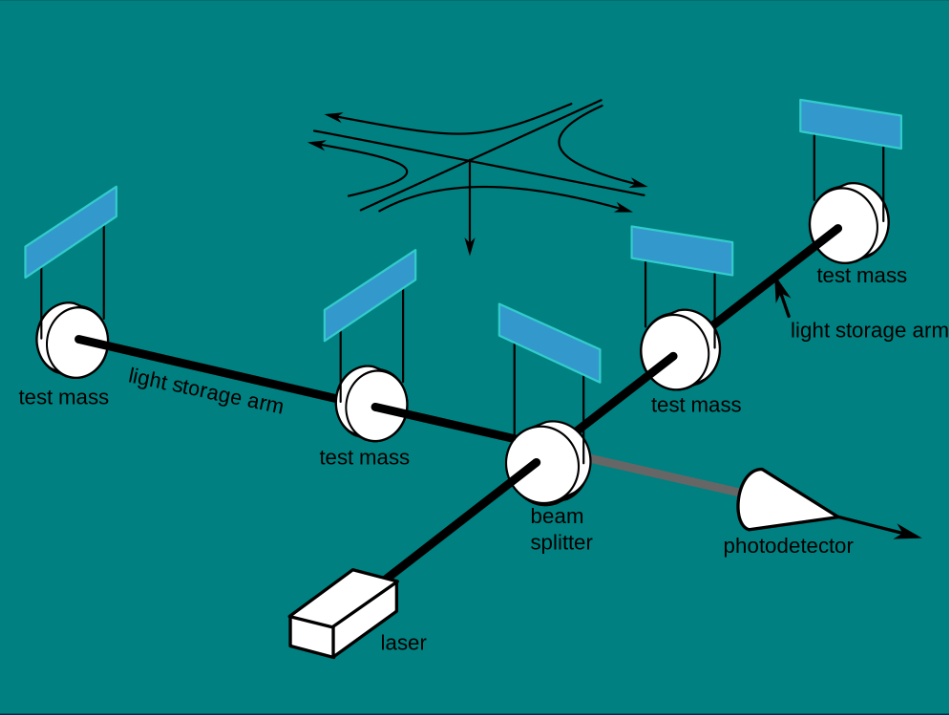
\includegraphics[width=0.7\linewidth]{1_grav}
	\caption{Пример детектора гравитационных волн (как интерферометр Майкельсона)}
	\label{fig:1_grav}
\end{figure}

Для регистрации гравитационных волн используются лазерные интерферометры, подобные интерферометру Майкельсона (см. рисунок \ref{fig:1_grav}). Принцип метода состоит в том, что гравитационная волна вызывает в установке прилив, при этом одно плечо интерферометра будет растягиваться, а другое --- сжиматься (меняются расстояния между свободно подвешенными зеркалами, между которыми «бегают» лазерные лучи). Этот эффект приведет к изменению интерференционного сигнала на детекторе, и его можно зарегистрировать.

Длина гравитационных волн, как правило, является довольно большой (она порядка размера того, что её излучает; в случае слияния чёрных дыр речь идёт о величинах порядка 100 км и больше). Поэтому для их детектирования в конструкцию интерферометра добавляют дополнительные зеркала (прозрачные на 0.1\%), которые как бы «запирают» свет внутри плеч, чтобы он успел «почувствовать» их влияние.

\subsection{Детекторы нейтрино}

Нейтрино — фундаментальные элементарные частицы, участвующие в слабом взаимодействии. Они очень плохо взаимодействуют с веществом, потому что не имеют электрического заряда, а также не участвуют в сильном ядерном взаимодействии.

Рассмотрим два типа детекторов нейтрино. Принцип действия первого детектора основан на том, что нейтрино, попав в ядро какого-либо атома, превращает это ядро в изотоп другого элемента, причём довольно атипичный. Пример: превращение хлора-37 в аргон-37 в результате бета-распада. Таким образом, для эксперимента берется большой объем хлорсодержащего вещества, а спустя некоторое время из него извлекается аргон-37, количество которого соответствует прошедшим в объеме детектора взаимодействиям нейтрино с хлором. Проблема такого способа регистрации нейтрино в том, что полностью теряется какая-либо информация об их направлении. К счастью, для нейтрино относительно низких энергий поблизости находится один-единственный источник --- Солнце.

Данный недостаток компенсируется водными детекторами. В них рабочим телом является вода, заполняющая огромную цистерну. Рассеиваясь на электронах, нейтрино передает им энергию, а электроны, двигаясь быстрее скорости света в воде, испускают черенковское излучение, которое регистрируется фотоумножителями, покрывающими стенки цистерны. Такие детекторы могут установить и направление прихода нейтрино (надо смотреть на частицы, которые идут снизу вверх, т.к. только нейтрино может пройти Землю наскозь), что дает возможность точно определить, что их источник --- Солнце или, например, вспышка сверхновой в нашей Галактике.

